% Paper E, JOURNAL OF INFORMETRICS version (Elsevier elsarticle, author-year).
% Text comes from ../../content/ (central version); only layout and journal-specific placement live here.
% JOI guide not reachable by script (403); user confirmed single-anonymized review on 2026-11-26.
% Author-confirmed JOI requirements (2026-11-27): abstract <=200 words; separate editable highlights, 3-5 x <=85.
% Elsevier AI policy read 2026-11-27; image-code assistance disclosed in captions as well as Methods/declaration.
% Upload the identified source package from build_submission.sh; keep \anonfalse and the public GitHub link.
% Build locally: tectonic -X compile main.tex (Elsevier compiles with pdflatex + bibtex).
\documentclass[preprint,12pt,authoryear]{elsarticle}
\usepackage{graphicx}
\usepackage{amsmath,amssymb}
\usepackage{booktabs}
\usepackage{array}
\usepackage{placeins}
\usepackage{lineno}
\usepackage{xcolor}
\usepackage{xurl}
\usepackage[hidelinks]{hyperref}
\setlength{\emergencystretch}{1.5em}
\newcommand{\todo}[1]{\textcolor{red}{[TODO: #1]}}
\newif\ifanon\anonfalse
\graphicspath{{../../figures/}}
% Paper E metadata (journal-neutral); title approved by the author on 2026-11-26.
\newcommand{\papertitle}{Do retracted papers look disruptive? The CD index before retraction on the open biomedical citation graph}
\newcommand{\papershorttitle}{Disruption of retracted papers}
\newcommand{\paperkeywords}{disruption index; CD index; retraction; research integrity; paper mills; OpenCitations}

\journal{Journal of Informetrics}
\biboptions{authoryear}
\renewcommand{\appendixname}{Appendix}

\begin{document}
\begin{frontmatter}
\title{\papertitle}
\ifanon
\author{Anonymous author}
\else
\author[msft]{Hossein Mohasel Arjomandi\corref{cor}}
\ead{hosseinm@microsoft.com}
\cortext[cor]{Corresponding author.}
\affiliation[msft]{organization={Microsoft}, addressline={One Microsoft Way}, city={Redmond}, state={WA},
postcode={98052-7329}, country={USA}}
\fi

\begin{abstract}
The consolidation--disruption (CD) index is used in research evaluation, but how it scores papers later retracted is
unclear. On OpenCitations linked to PubMed, we compared late-retracted biomedical papers with never-retracted controls
from the same journal and year. Late-retracted means that the first retraction notice occurred at least six calendar
years after publication. The pre-specified five-year index (CD$_5$) showed a small mean gap (0.0002) and no clear
top-tier excess, but positive scores were more common (odds ratio 1.23, 95\% confidence interval 1.13--1.34).
An exploratory analysis, planned after these results were known, found that papers citing a retracted paper were
less likely to also cite its references: on average, 65.5\% versus 68.8\%.
CD$_5$ compresses this contrast because papers citing only the references dominate its denominator.
The variant without that term (DI$_{nok}$) had a mean gap of 0.067 (0.034--0.095).
As a robustness check, excluding notice, comment/letter and retracted citing records increased the gap to 0.082.
The filtered contrast persisted with reference and citation adjustment
and after excluding the ten journals with the most late-retracted papers in the study.
For unfiltered scores, a small topic-matched subset did not establish a gap.
CD$_5$ can look neutral while DI$_{nok}$ scores late-retracted papers higher within journal/year comparisons.
Researchers and bulk score providers should end scoring windows before the first retraction notice,
with notice records removed.

\end{abstract}

\begin{keyword}
disruption index \sep CD index \sep retraction \sep research integrity \sep paper mills \sep OpenCitations
\end{keyword}
\end{frontmatter}
\linenumbers

\section{Introduction}\label{sec:intro}

The CD index \citep{funk2017dynamic} compares the later papers that cite a focal paper with the later papers that cite
the focal paper's references. Citing papers that ignore the references push the score towards $+1$, and the paper is
called disruptive; citing papers that also cite them push it towards $-1$, and the paper is called consolidating;
papers that cite only the references pull the score towards zero. The index became widely known through studies of
team size \citep{wu2019large} and of a decline in disruptiveness across science and technology \citep{park2023papers}.
An inventory lists 105 studies that bear on whether innovation is becoming less disruptive
\citep{wu2026inventory}, and recommendations have been made for using the index in research evaluation
\citep{chen2025thresholds}. The index is also debated: records without references can drive measured trends
\citep{holst2024artefacts,holst2026partially,park2026reply}, citation inflation biases it
\citep{petersen2024inflation,petersen2025reanalysis}, and its values depend on the data source
\citep{leibel2023overview,xu2025alternative}.

A question that matters for both uses has not been answered: how does the index score papers that are later
retracted? Retractions for paper-mill production have grown quickly: the Retraction Watch snapshot used here records
11,716 such papers, with at most four retraction notices per year before 2020 and 6,782 in 2023 alone. If fabricated
or mass-produced papers scored as disruptive, an evaluation that rewards disruption would also reward them; if they
scored as consolidating, the index might carry a signal that integrity screening could use. The closest prior work
studied other units: questionable publications were less disruptive than comparable publications
\citep{you2022questionable}, and a disruption measure computed for MeSH concepts differed between the concepts used to
annotate retracted and non-retracted papers in most years \citep{copara2024mesh}. Neither compared the scores of the
retracted papers themselves with those of comparable papers, measured before the retraction.

Opposite expectations are plausible. Fabricated or falsified results can report findings that later work cites as new
evidence without engaging the literature the paper built on; such papers would score as disruptive. Paper-mill products
follow templates and standard methods; if they are cited mainly by similar products that cite the same standard works,
they would score as consolidating. The retraction itself may also change how a paper is cited: citations fall sharply
after a retraction \citep{azoulay2015retractions}, retraction notices appear among the citing items
\citep{hsiao2021continued}, and scores computed over windows that include these years may describe the retraction
rather than the paper.

This study answers the question on the open biomedical citation graph. The comparison has three features. First, it is
temporal: retracted papers enter the main analysis only if the retraction came after their five-year scoring window
closed, so the score reflects how the paper was cited while it was still part of the record. Second, each retracted
paper is compared with never-retracted papers from the same journal and publication year. Third, the design, the
reason classes and every pre-planned analysis were written down before any score was computed. Analyses added later
are labelled exploratory; they include interval bounds, a review positive control, a variant of the index without
its $n_k$ term, reference-length diagnostics and a comparison of citing papers around the retraction notice.

Contributions:
\begin{itemize}
\item A paper-level measurement of the CD index for retracted papers scored before their retraction, overall and by
retraction reason (paper mill, misconduct, honest error), for 4,587 papers, of which 4,586 are compared with 31,662
scored controls in 2,239 journal--year strata, with a post hoc extension to 7,349 scored papers, of which 7,348 are compared.
\item Bounds on the small mean difference and no unadjusted top-tier excess in the pre-specified five-year analysis,
alongside a positive-score shift; the post hoc three-year window leans toward a modest top-tier excess.
\item Evidence that the index hides a difference in how retracted papers are cited: papers that cite a retracted paper
are less likely to also cite its references, and at equal reference length retracted papers reach the top tier more often.
\item Evidence that scores including the years after the notice are shifted by notice records and by a gap that widens
around the notice, with a practical recommendation for evaluators.
\item Open code, run records and specification files that let the analysis be repeated on the public data.
\end{itemize}

\section{Related work}\label{sec:related}

\paragraph{The CD index and its debates} \citet{funk2017dynamic} introduced the index for patents, using citations in
the first five years after a patent's issue; \citet{wu2019large} and \citet{park2023papers} applied it to tens of
millions of papers. \citet{wu2019large} call papers in the top 5\% of the disruption distribution highly disruptive.
\citet{park2023papers} reported that papers and patents have become less disruptive over the decades they studied,
with PubMed among the robustness datasets. \citet{holst2024artefacts} argued that records without references, which
receive CD$_5 = 1$ whenever they are cited, are hidden drivers of that decline; the published comment states that such
artefacts can partially drive it \citep{holst2026partially}, and the original authors dispute an artefact-based
explanation \citep{park2025robust,park2026reply}. \citet{petersen2024inflation} showed that citation inflation,
including the growth of reference lists, biases the index, and \citet{petersen2025reanalysis} found that trends
controlled for it show a small increase in 2005--2015 that they describe as ``at the level of noise.''
\citet{leibel2023overview} review the index
family, its variants and its limitations, and \citet{lin2026displacement} interpret the index as capturing the
displacement of a paper's most cited reference.

\paragraph{Variants and data sources} Several variants change the terms of the index. The variant without $n_k$, the
number of papers that cite only the references, was proposed by \citet{wuyan2019solo} and studied as DI$_1^{nok}$ by
\citet{bornmann2020convergent}, who questioned the function of $n_k$ and explained how it compresses scores.
\citet{leydesdorff2021revision} proposed revised indices DI$^*$ and DI$^\#$.
Our exploratory comparison examines what this known denominator issue means for late-retracted papers.
Disruption has been computed at scale on Dimensions \citep{sixt2024dimensions} and on
OpenCitations \citep{jiang2024opencitations}, and compared across Web of Science, Dimensions and OpenCitations
\citep{xu2025alternative,crossdi2025}. Biomedical applications include an analysis of PubMed papers
\citep{sheng2023prior} and disruption measures for MeSH concepts \citep{copara2024mesh}. \citet{deng2025persistent}
identify persistently disruptive papers, which are not themselves disrupted by the papers that cite them.

\paragraph{Disruption and questionable work} Two studies link disruption measures to research integrity.
\citet{you2022questionable} found that questionable publications, as they defined them, were less disruptive and less
influential than comparable publications. \citet{copara2024mesh} propagated article disruption scores to MeSH concepts
and aggregated concept metrics for papers. Their disruption-specific comparison differed between retracted and
non-retracted papers in seven of eight years; the overall relevance composite, combining informativeness, usefulness,
disruptiveness and influence, was also reported to differ ($p<0.05$). Neither compares matched papers on their own paper-level CD
scores, and neither scores them
before the retraction. The literature search for this study, which included the 105-study inventory of
\citet{wu2026inventory}, found no such comparison.

\paragraph{Retractions in citation networks} Retracted papers cluster within citation networks
\citep{feng2024molbio,lou2026beyond}, and papers that cite them are retracted more often \citep{lou2026beyond}.
A prospective analysis on the same open citation snapshot found that citing papers retracted by the predictor cutoff
was associated with later retraction within journal and year \citep{arjomandi2026prospective}; it used the same linked
Retraction Watch dataset \citep{arjomandi2026retracteddata}, but did not analyse disruption.
Paper-mill retractions share characteristics \citep{candal2022papermills}, tools flag papers that cite retracted work
\citep{cabanac2024chain} and other problematic papers \citep{cabanac2022pps}, and retraction can be predicted to a
limited extent from text and metadata \citep{fletcher2025predicting}. Citations to a paper fall sharply after its
retraction \citep{azoulay2015retractions}, and retraction notices themselves appear among the citing items of retracted
papers \citep{hsiao2021continued}. None of these studies uses the disruption index.

\section{Data and methods}\label{sec:methods}

\subsection{Data}
\paragraph{Citation graph} The graph is the January 2024 OpenCitations snapshot distributed as parsed tables by
\citet{arjomandi2024dataset} \citep[see also][]{peroni2020opencitations}. Publication years, identifiers and journals
come from OpenCitations Meta \citep{massari2024meta,ocmeta2024dump}. Measured by the monthly count of citing papers,
the snapshot is effectively complete to about September 2023. A paper is \emph{biomedical} if it has a PMID in Meta or
its DOI appears in the PubMed 2026 baseline, from which publication types and comment/correction links are also taken.

\paragraph{Retractions} Retraction labels come from the Retraction Watch database distributed by Crossref
\citep{rittman2025rw}, in the repository snapshot of 30 October 2026 (62,735 retracted papers). Papers were linked to graph
nodes by DOI or PMID; 52,254 of the 62,735 (83.3\%) were matched, giving 53,170 graph nodes. The linked table is
public \citep{arjomandi2026retracteddata}. The date of the first retraction notice and the union of the reasons given
by Retraction Watch are kept per paper; reinstated papers are excluded.

\paragraph{Reason classes} Each retracted paper receives one class, assigned in this order: \emph{paper mill} (reason
``Paper Mill''); \emph{misconduct} (fabrication or falsification, manipulation of images, data or results, plagiarism,
duplicated images, compromised peer review, rogue editor, forged authorship or affiliation, computer-generated
content, hoax papers, or an official misconduct finding); \emph{honest error} (any ``Error in'' or ``Error by''
reason, results not reproducible, contaminated materials or cell lines, ``Doing the Right Thing''); and \emph{other}
(everything else, including notices with limited information). The full list of reason strings is in the
specification file (see the data and code availability statement).

\subsection{Populations}
\paragraph{Eligible papers} Biomedical papers published 2000--2017 with a journal in Meta, at least one reference in
the graph, and no duplicate DOI record. The year limit ensures that the five-year window ends by 2022, inside the
complete part of the snapshot. Papers without references are excluded: their index equals 1 whenever they are cited
and is undefined otherwise, and they are the records behind the CD$_5 = 1$ artefact discussed by
\citet{holst2024artefacts}. Of 12,522,210 biomedical papers from 2000--2017 with a journal, 341,432 (2.7\%) have no
reference in the graph, leaving 12,180,778 eligible papers.

\paragraph{Retracted papers} Eligible papers matched to a retraction: 10,450. The \emph{primary set} contains the
4,587 papers whose first retraction notice is dated after 31 December of the fifth year after publication, so that the
whole scoring window precedes the retraction. The 5,863 papers retracted earlier form, together with the primary set,
the \emph{secondary set} used in a robustness check.

\paragraph{Controls} For every retracted paper, five eligible papers from the same journal and publication year that
are neither in Retraction Watch nor flagged as retracted in PubMed. Within a stratum, controls are the papers with the
lowest value of a fixed hash of their identifier (seed 20261109), which makes the draw deterministic. This gives
52,147 controls in 5,458 journal $\times$ year strata; four strata (four retracted papers) have no eligible control.
This pool is drawn for all 10,450 retracted papers, not just the 4,587 primary-set papers. A comparison uses only the
controls with a defined score in strata containing scored papers of the compared set. The primary analysis uses
2,239 strata containing 4,586 primary-set papers and 31,662 scored controls.

\paragraph{Reference sample} A deterministic 0.2\% sample of all eligible papers (24,491 papers) provides the
yearly distribution of the index, from which the top-5\% and top-1\% thresholds are taken.

\paragraph{Post hoc population} The same rules applied to papers published 2000--2019 with a three-year window give
13,661 retracted papers (7,350 retracted after their window), 68,190 controls and a reference sample of 28,784 papers.
It contains every paper of the population above.

\subsection{The CD index}\label{sec:score}
For a focal paper $f$ published in year $t$ with references $R(f)$ in the graph, let $A$ be the papers published in the
window that cite $f$, and $B$ the papers published in the window, other than $f$, that cite at least one paper in
$R(f)$. With $n_i = |A \setminus B|$ (citing papers that cite none of the references), $n_j = |A \cap B|$ (citing
papers that also cite at least one reference) and $n_k = |B \setminus A|$ (papers that cite only the references),
\begin{equation}
\mathrm{CD}(f) = \frac{n_i - n_j}{n_i + n_j + n_k},
\end{equation}
undefined when the denominator is zero \citep{funk2017dynamic,park2023papers}. Self-loops are ignored.
\citet{park2023papers} measure the index five years after each paper's publication year. The main window (CD$_5$)
covers the citing years $t$ to $t+5$; because year-level data cannot order the focal paper and other papers of the same
year, those papers are included. The reference implementation of the index counts only citing works with a later
timestamp than the focal work\footnote{Software \texttt{cdindex} by R.~J. Funk,
\url{https://github.com/russellfunk/cdindex}, file \texttt{src/cdindex.c} at commit \texttt{4eece64}.}, which with
year-level timestamps corresponds to the citing years $t+1$ to $t+5$; this window is used in robustness check (d).

The post hoc variant without $n_k$,
\begin{equation}
\mathrm{DI}_{nok}(f) = \frac{n_i - n_j}{n_i + n_j},
\end{equation}
was proposed by \citet{wuyan2019solo} and studied as DI$_1^{nok}$ by \citet{bornmann2020convergent}. It depends only on
the papers that cite $f$ and is defined when there is at least one; $(1 - \mathrm{DI}_{nok})/2$ is the share of
citing papers that also cite a reference. CD and DI$_{nok}$ always have the same sign.

The score script reads only the list of focal papers and their years; it never reads retraction labels. Its output
(86,950 papers) was hashed (SHA-256) before the evaluation script joined the labels, and the evaluation script checks
the hash. An implementation in DuckDB \citep{raasveldt2019duckdb} was tested against a brute-force count on random
graphs (1,200 focal papers, both windows, identical counts). For the before-and-after comparison, a second label-free
script counted the citing papers of each focal paper by citing year; its sums over the scoring windows equal the frozen
counts for all 110,462 papers of both populations, and its output was hashed before labels were joined.

\paragraph{Pre-specification record} The unchanged specification is \texttt{SPEC.md}, committed in the then-private
project repository on 10 November 2026 at 04:02:19 UTC (Git commit
\texttt{293755b1cb7087d6f226d6f96f4b97cb0148e4c5}). Its SHA-256,
\nolinkurl{1403d0d13d35bd32c40ede1be24833ab15e7977edb2f56c2128ef8823373ad31},
is recorded in the score run's \texttt{run.json}, which reports a start time of 06:12:02 UTC the same day
(\texttt{e03\_cd5\_20261110\_01}); the evaluation run records the same hash. These files and provenance are available
with the code. Git dates and local run records are not an independent registry timestamp, so the design is described
as pre-specified, not publicly pre-registered.

\subsection{Analyses}
All analyses below were specified before any score was computed, except those marked post hoc. The plan of each post
hoc analysis, with its margins and expected directions, was recorded before it was run.
\begin{itemize}
\item \textbf{RQ1 (primary):} the mean difference in CD$_5$ between retracted papers and their controls within
journal $\times$ year strata, averaged over retracted papers, with a 95\% interval from 2,000 bootstrap resamples of
strata; and the Mantel--Haenszel odds ratio \citep{mantel1959} for a positive score (CD$_5 > 0$), with the
Robins--Breslow--Greenland variance \citep{robins1986estimator}.
\item \textbf{RQ2:} the same by reason class.
\item \textbf{RQ3:} the share of papers at or above the 95th and 99th percentiles of CD$_5$ in their publication year
(from the reference sample), with Wilson intervals \citep{wilson1927}, and the stratified odds ratio for reaching them.
\item \textbf{Robustness (pre-specified):} (a) without CD$_5 = 1$ papers; (b) without reviews (PubMed publication
types Review, Systematic Review, Meta-Analysis); (c) strata further split by deciles of reference count; (d) window
$t+1$ to $t+5$; (e) the secondary set; (f) papers with at least five citations in the window.
\item \textbf{Post hoc, first round:} (P1) reference and citation counts by group; (P2) a three-year window (CD$_3$)
for papers published 2000--2019, which adds paper-mill papers from 2018--2019, with the primary set defined by a
retraction after the third year.
\item \textbf{Post hoc, second round:} (P3) equivalence tests: two one-sided tests \citep{schuirmann1987tost,
lakens2017equivalence} with margins of $\pm 0.1$ standard deviations of the score in the reference sample for mean
differences and 0.80--1.25 for odds ratios; these post hoc margins are conventions, not validated thresholds for the CD
index. Equivalence is shown if the 90\% interval lies inside the margin; the smallest supported symmetric margin is
reported so readers can apply a different threshold. (P4) A positive control: reviews compared with the other
never-retracted controls of the same journal and year, expected to be more consolidating because papers citing a
review often also cite the work it reviews. (P5) RQ1--RQ3 with DI$_{nok}$. (P6) Before and after the notice: for
retracted papers of the 2000--2019 population with retraction year $R$ between $t+1$ and 2021, the change in
DI$_{nok}$ from the citing years $R-3$ to $R-1$ (not before $t$) to the years $R+1$ to $R+3$ (not after 2022),
minus the mean change of their stratum's controls over the same years, for papers with at least one citing paper in
both periods, with year $R$ and notice records excluded.
(P7) The sign shift: papers without citing papers in the window, odds ratios among cited papers only, and conditional
logistic regression within journal $\times$ year strata with $\log(1+\text{references})$ and
$\log(1+\text{citing papers in the window})$ as covariates. (P8) Editorial notices: citing records that PubMed
types as retraction notices, published errata or expressions of concern, or that carry the corresponding links
(RetractionOf, ErratumFor, ExpressionOfConcernFor), and robustness check (e) without them.
\item \textbf{Post hoc, third round:} (P9) checks of P6 for an earlier trend: a placebo notice three years before the
real one, and yearly means on a balanced set of papers; (P10) the size of $n_k$.
\item \textbf{Post hoc, fourth round (descriptive):} (P11) the controls behind the primary comparisons: their number in
the strata used, and their shares above zero and above the yearly thresholds, with each stratum weighted by its
retracted papers as for the mean difference (95\% interval from 2,000 bootstrap resamples of strata).
\end{itemize}
Only group-level results are reported. No per-paper score of a non-retracted paper is released.

\paragraph{Software and AI assistance} The analyses ran in Python 3.11 with DuckDB 1.5, pandas 3.1, NumPy 2.4, SciPy
1.17 and statsmodels 0.15 on one cloud machine; figures were drawn with Matplotlib 3.10 from the run records. The
analysis and figure scripts were written with the help of a generative AI assistant (Claude Opus 5.5, Anthropic) under
the author's direction. Every counting step was tested against brute-force counts on random graphs, each evaluation
script first reproduces the earlier estimates it builds on, and all scripts and run records are public
(see the data and code availability statement).

\begin{figure}[!htbp]
\centering
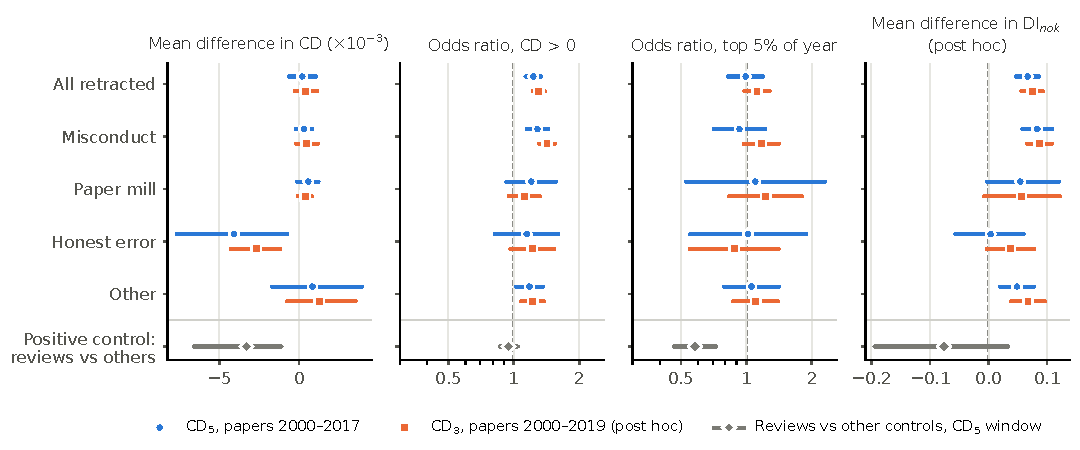
\includegraphics[width=\linewidth]{fig1_forest}
\caption{Retracted papers versus controls from the same journal and publication year, by retraction reason, and the
positive control (grey diamonds: reviews versus the other never-retracted controls, CD$_5$ window).
Reading across rows, panels 1--3:
stratified mean difference in the CD index ($\times 10^{-3}$) and Mantel--Haenszel odds ratios for a positive score
and for reaching the top 5\% of the publication year. Panel 4: the unfiltered mean difference in
DI$_{nok}$, the variant without $n_k$ (post hoc), before the citing-record sensitivity.
Bars: 95\% intervals. Panel 1 retains the pre-specified journal--year bootstrap;
panel 4 resamples whole journals, as does Table~\ref{tab:citers}.
Dashed lines mark the null (0 for mean gaps, 1 for odds ratios).
Circles: CD$_5$, papers 2000--2017, retracted after the five-year window
(pre-specified). Squares: CD$_3$, papers 2000--2019, retracted after the three-year window (post hoc).
Claude Opus 5.5 (Anthropic) assisted plotting code; GitHub Copilot CLI 1.0.116 (GitHub) assisted code and layout
revisions. The plotted values come directly from the reproducible analysis records.}
\label{fig:forest}
\end{figure}

\section{Results}\label{sec:results}

\subsection{Scores and thresholds}
CD$_5$ is defined for 86,904 of the 86,950 scored papers; the other 46 (25 controls, two papers retracted inside their
window and 19 papers of the reference sample) have no paper in the window that cites them or one of their references,
so $n_i+n_j+n_k=0$. Thus, 52,122 of the full pool of 52,147 controls have a defined score; the 25 undefined scores
are excluded, not treated as zero.
The distribution is concentrated near zero: in the scored set the 5th, 50th and 95th
percentiles are $-0.0218$, $-0.0010$ and $0.0059$. The large $n_k$ term compresses the scores
(\ref{sec:appendix}). Papers without a citing paper in the window but with $n_k>0$ score exactly zero. CD$_5 = 1$ is
rare (0.04\% of defined scores) because papers without references are excluded. In the reference sample, the yearly
top-5\% threshold falls from 0.021 (2000) to between 0.005 and 0.006 (2014--2017), and the top-1\% threshold from 0.13
to between 0.04 and 0.06. The mean CD$_5$ per publication year stays between $-0.0049$ and $0.0009$.

\subsection{RQ1: retracted papers versus matched controls}
The comparison population is shown in Fig.~\ref{fig:population}. Control percentages below use its defined-score
comparison group, with each stratum weighted by its number of scored primary-set papers, as for the mean difference.
The stratum-weighted mean CD$_5$ is $-0.002165$ for retracted papers and $-0.002363$ for their controls, a difference of
$0.00020$ (95\% CI $-0.00061$ to $0.00109$).
The post hoc 90\% interval, $-0.00051$ to $0.00093$, rules out absolute
mean differences larger than 0.00093, about 28\% of the difference between reviews and other papers (below).
Retracted papers have a positive score somewhat
more often within the comparison strata (923 of 4,586, 20.1\%, against 17.3\% of their controls, 95\% bootstrap CI
16.0--18.6; stratified odds ratio 1.23, 1.13--1.34).

\subsection{RQ2: reason classes}
The mean differences for misconduct (2,742 compared papers) and paper-mill production (276) are small
and their 95\% intervals include zero (Table~\ref{tab:main}). The post hoc 90\% intervals are $-0.00010$ to $0.00074$
and $0.00001$ to $0.00111$, respectively.
Their odds of reaching the top 5\% are close to one but imprecise (Table~\ref{tab:main},
Fig.~\ref{fig:forest}). None of the 276 paper-mill papers reaches the top 1\%. Papers retracted for honest error (294)
score lower than their controls (difference $-0.0041$, $-0.0077$ to $-0.0007$), that is, they are slightly more
consolidating.

\subsection{RQ3: the most disruptive papers}
In the pre-specified five-year analysis, retracted papers are not over-represented among the most disruptive papers of their year
(Table~\ref{tab:main}). 3.1\% of them (2.6--3.6) reach the top-5\% threshold, against 3.1\% (2.8--3.5) of their
controls, weighted in the same way; within strata the odds ratio is 0.99 (0.83--1.20). For the top 1\%, 17
retracted papers (0.37\%, 0.23--0.59) reach the threshold, against 0.54\% (0.43--0.66) of their controls; the odds
ratio of 0.67 (0.40--1.12) is imprecise. Both groups reach the yearly thresholds less often than
the nominal 5\% and 1\%: they come from the journals in which retractions occur, whereas the thresholds come from the
reference sample of all eligible papers.

\begin{table}[t]
\centering
\caption{CD$_5$ of retracted papers (primary set) versus controls from the same journal and year, by reason class.
Diff.: stratified mean difference ($\times 10^{-3}$, 95\% bootstrap CI). OR: Mantel--Haenszel odds ratio (95\% CI).
$n$: retracted papers in strata with a defined control score, not all scored retracted papers.}
\label{tab:main}
\resizebox{\linewidth}{!}{%
\begin{tabular}{lrrrrr}
\toprule
 & $n$ & Diff. ($\times10^{-3}$) & OR, CD$_5>0$ & OR, top 5\% & Top 1\% ($n$) \\
\midrule
All retracted & 4,586 & 0.20 ($-0.61$, 1.09) & 1.23 (1.13, 1.34) & 0.99 (0.83, 1.20) & 17 \\
Misconduct & 2,742 & 0.32 ($-0.21$, 0.82) & 1.29 (1.15, 1.44) & 0.93 (0.71, 1.22) & 5 \\
Paper mill & 276 & 0.58 ($-0.14$, 1.23) & 1.20 (0.93, 1.57) & 1.10 (0.53, 2.29) & 0 \\
Honest error & 294 & $-4.08$ ($-7.68$, $-0.73$) & 1.15 (0.82, 1.60) & 1.02 (0.55, 1.88) & 2 \\
Other & 1,274 & 0.84 ($-1.72$, 3.97) & 1.18 (1.02, 1.36) & 1.06 (0.79, 1.41) & 10 \\
\bottomrule
\end{tabular}}
\end{table}

\subsection{Robustness}
Table~\ref{tab:rob} gives the pre-specified checks. Excluding CD$_5 = 1$ papers (a), reviews (b) or using the window
$t+1$ to $t+5$ (d) leaves the results unchanged. Three checks move them. Splitting strata by reference-count decile
(c) gives a positive mean difference and an odds ratio of 1.47 (1.15--1.88) for the top 5\%; this check keeps only the
3,664 retracted papers that have a control in the same decile. The reference-length analysis below describes an
imbalance in the direction of this shift. Restricting to papers with at least five citations in the window (f) gives a
small positive mean difference. Including the 5,863 papers retracted inside their window (e) raises the odds ratio for
a positive score from 1.23 to 1.50 (1.42--1.58), while the top-5\% odds ratio stays at 1.00.

\begin{table}[t]
\centering
\caption{Robustness checks for the primary set (CD$_5$) and the post hoc three-year window (CD$_3$).
Diff.\ in units of $10^{-3}$; all estimates have 95\% intervals in parentheses.}
\label{tab:rob}
\resizebox{\linewidth}{!}{%
\begin{tabular}{lrrr}
\toprule
\multicolumn{4}{l}{CD$_5$, 2000--2017} \\
Check & Diff. & OR, CD$>0$ & OR, top 5\% \\
\midrule
Main analysis & 0.20 ($-0.61$, 1.09) & 1.23 (1.13, 1.34) & 0.99 (0.83, 1.20) \\
(a) no CD $=1$ & 0.05 ($-0.50$, 0.59) & 1.23 (1.13, 1.33) & 0.99 (0.82, 1.19) \\
(b) no reviews & 0.14 ($-0.74$, 1.18) & 1.23 (1.12, 1.34) & 0.98 (0.81, 1.19) \\
(c) + reference deciles & 1.23 (0.39, 2.23) & 1.38 (1.24, 1.53) & 1.47 (1.15, 1.88) \\
(d) window from $t+1$ & 0.31 ($-0.63$, 1.35) & 1.24 (1.14, 1.35) & 1.01 (0.84, 1.21) \\
(e) all retracted & 1.44 (0.78, 2.21) & 1.50 (1.42, 1.58) & 1.00 (0.90, 1.12) \\
(f) $\ge 5$ citations & 0.62 (0.07, 1.15) & 1.28 (1.17, 1.41) & 1.09 (0.88, 1.35) \\
\midrule
\multicolumn{4}{l}{CD$_3$, 2000--2019 (post hoc)} \\
Check & Diff. & OR, CD$>0$ & OR, top 5\% \\
\midrule
Main analysis & 0.39 ($-0.27$, 1.14) & 1.30 (1.22, 1.39) & 1.12 (0.98, 1.28) \\
(a) no CD $=1$ & 0.32 ($-0.17$, 0.83) & 1.30 (1.22, 1.39) & 1.12 (0.98, 1.28) \\
(b) no reviews & 0.39 ($-0.32$, 1.17) & 1.31 (1.22, 1.40) & 1.13 (0.98, 1.30) \\
(c) + reference deciles & 1.26 (0.52, 2.02) & 1.33 (1.23, 1.44) & 1.46 (1.23, 1.73) \\
(d) window from $t+1$ & 0.54 ($-0.22$, 1.38) & 1.32 (1.24, 1.40) & 1.15 (1.01, 1.31) \\
(e) all retracted & 1.27 (0.67, 1.90) & 1.54 (1.47, 1.61) & 1.16 (1.06, 1.26) \\
(f) $\ge 5$ citations & 0.78 (0.23, 1.36) & 1.39 (1.29, 1.49) & 1.32 (1.12, 1.56) \\
\bottomrule
\end{tabular}}
\end{table}

\subsection{Exploratory: why the sign shift?}
\paragraph{A review positive control}
Reviews among the never-retracted controls score lower than the other controls of the same journal and year: the mean
difference in CD$_5$ is $-0.0033$ ($-0.0066$ to $-0.0011$), and reviews reach the top 5\% (odds ratio 0.58,
0.47--0.72) and the top 1\% (0.39, 0.21--0.73) much less often (6,032 reviews, 4,832 of them in the 2,083 strata that
also contain other controls; Fig.~\ref{fig:forest}). The design therefore detects a contrast expected from the
construction of the index, with sample sizes similar to those of the main analysis.
The odds ratio for a positive CD$_5$ is 0.95 (0.86--1.04), and the mean DI$_{nok}$ difference is
$-0.076$ ($-0.195$ to $0.033$; 4,736 compared reviews). Both intervals include the null: the positive control
detects the CD$_5$ mean and top-tier contrasts, but not a clear sign or DI$_{nok}$ mean contrast.
The bootstrap resamples weighted journal--year contrasts, whose values and weights differ between the review and
retraction comparisons; similar numbers of papers therefore do not imply similar interval widths.

\paragraph{Citation composition}
The variant without $n_k$ reveals a citation-composition difference that CD$_5$ compresses.
After excluding notice, Comment/Letter and retracted citing records, the mean DI$_{nok}$ gap is 0.082
(95\% journal-bootstrap CI 0.049--0.110; Table~\ref{tab:citers}).
The matched means are $-0.2995$ for retracted papers and $-0.3811$ for controls:
on average, 65.0\% of papers citing a retracted paper also cite a reference, against 69.1\% for controls.
The comparison retains 4,504 retracted papers and 30,389 controls in 2,190 strata and 972 journals
(Fig.~\ref{fig:population}).

Excluding these citing records increases rather than removes the gap. With the same journal-bootstrap design,
the unfiltered gap is 0.067 (0.034--0.095), becomes 0.069 after notice removal and 0.070 after also removing
comments and letters. The full filter makes 13 previously defined primary scores undefined; comparison strata
are re-evaluated, not filled with zeros.
Adjusting the DI$_{nok}$ mean for log reference and remaining citing-paper counts within strata gives a gap
of 0.097 (0.065--0.127). Excluding the ten journals with most original primary-set retractions reduces the filtered
gap to 0.053 (0.033--0.074); with both covariates it is 0.070 (0.049--0.091).
Class-specific and population diagnostics are in \ref{sec:appendix}.

CD and DI$_{nok}$ have the same sign. In the original counts, excluding uncited papers leaves a positive-score
odds ratio of 1.20 (1.11--1.31); holding reference and citation counts fixed gives 1.32 (1.21--1.43).
These sign models and the unfiltered intervals in Fig.~\ref{fig:forest} are retained separately in
Table~\ref{tab:posthoc}. DI$_{nok}$ cannot define a top tier: its yearly 95th and 99th percentiles equal 1.

\begin{table}[!htbp]
\centering
\caption{Exploratory citing-record sensitivity of the DI$_{nok}$ mean. All intervals are 95\% whole-journal
bootstrap intervals; original journal--year matching is retained. Filters remove citing records, not focal references.
Adjusted rows are weighted within-stratum linear models. $n$: compared retracted papers.}
\label{tab:citers}
\small
\begin{tabular}{@{}>{\raggedright\arraybackslash}p{0.48\linewidth}lr@{}}
\toprule
Analysis & Mean gap (95\% CI) & $n$ \\
\midrule
CD$_5$ window: unfiltered & 0.067 (0.034, 0.095) & 4,517 \\
Exclude notices & 0.069 (0.037, 0.096) & 4,517 \\
Also exclude Comment/Letter & 0.070 (0.037, 0.098) & 4,513 \\
Also exclude retracted citing papers & 0.082 (0.049, 0.110) & 4,504 \\
Full filter, adjust log references & 0.094 (0.060, 0.124) & 4,504 \\
Full filter, also adjust log citations & 0.097 (0.065, 0.127) & 4,504 \\
Full filter, exclude top ten journals & 0.053 (0.033, 0.074) & 3,013 \\
Same exclusion, both covariates & 0.070 (0.049, 0.091) & 3,013 \\
CD$_3$ window: full filter & 0.090 (0.064, 0.114) & 7,088 \\
CD$_3$: also exclude top ten journals & 0.082 (0.064, 0.099) & 5,057 \\
\bottomrule
\end{tabular}
\end{table}

\subsection{Exploratory: reference length and the top tier}
The top-tier comparison is sensitive to reference length. In the conditional logistic regression, the odds ratio for
reaching the top 5\% of CD$_5$ is 0.99 without covariates and 1.42 (1.16--1.75) with $\log(1+\text{references})$;
adding $\log(1+\text{citing papers in the window})$ gives 1.19 (0.96--1.47). Short reference lists favour high scores
(coefficient $-1.64$ per unit of log references). The matched diagnostic, using the same log transformation
as this model, gives means of $\log(1+\text{references})$ of 3.6418 for the 4,586 compared retracted papers and 3.5575
for their 31,662 controls, weighted within strata. The difference is $+0.084$ (95\% strata-bootstrap CI
0.058--0.109). This imbalance pushes retracted papers' unadjusted scores down.
The corresponding matched difference in mean $\log(1+\text{citing papers})$ is $+0.311$ (0.280--0.341).

Restricting both groups by PubMed publication types retains the reference-length imbalance and reference-adjusted
top-tier excess. The filter, full estimates and population accounting are in \ref{sec:appendix}.

\subsection{Exploratory: what happens around the notice?}
Removing editorial notice records changes the primary positive-score estimate little, but reduces it for papers
retracted inside the scoring window (\ref{sec:appendix}).
Beyond notices, the citing papers change around the retraction. For 5,100 retracted papers
from 2000--2019 with citing papers before and after the notice, DI$_{nok}$ rose by 0.174 from the three years before
the notice year to the three years after it, against 0.100 for their controls over the same calendar years: a
difference in differences of 0.074 (0.050--0.097). Their citations fell from 3.9 to 2.6 per year, while those of the
controls rose from 3.1 to 4.7. The change began before the notice, as the placebo check confirms
(\ref{sec:appendix}).
In a separate balanced population of 3,083 papers, Figure~\ref{fig:event} plots the mean paired annual gap
in DI$_{nok}$: 0.053 (95\% CI 0.020--0.083) three years before the notice, 0.092 (0.059--0.124) in the notice year,
and 0.201 (0.162--0.242) two years after it. These estimates use 2,220, 2,440 and 1,982 defined pairs,
respectively; uncited annual scores are undefined.

\subsection{Exploratory: a shorter scoring window}
The shorter window admits more recent papers, including more paper-mill papers (population counts in \ref{sec:appendix}).
The mean difference remains small,
$0.00039$ ($-0.00027$ to $0.00114$), and the odds ratio for a positive score is 1.30
(1.22--1.39); top 5\% 1.12 (0.98--1.28); top 1\%
0.89 (0.63--1.28). Unlike the pre-specified five-year comparison, these post hoc top-5\% estimates lean toward a
modest excess: the odds ratios are 1.15 (1.01--1.31) when the window starts at $t+1$, 1.16 (1.06--1.26) for all
retracted papers, and 1.32 (1.12--1.56) among papers with at least five window citations (Table~\ref{tab:rob}).
For paper-mill papers the mean difference is $0.00039$ ($-0.00009$ to $0.00082$), the top-5\% odds
ratio 1.23 (0.83--1.81), and none of the 708 reaches the top 1\% (Fig.~\ref{fig:forest}).
The article-type restriction strengthens the apparent three-year top-tier excess, whereas author-name exclusions
attenuate it. Full estimates are in \ref{sec:appendix}; the excess is not clear under every sensitivity restriction.
The fully filtered DI$_{nok}$ mean gap remains positive in this window, including after the top-ten-journal
exclusion (Table~\ref{tab:citers}).




\begin{figure}[!htbp]
\centering
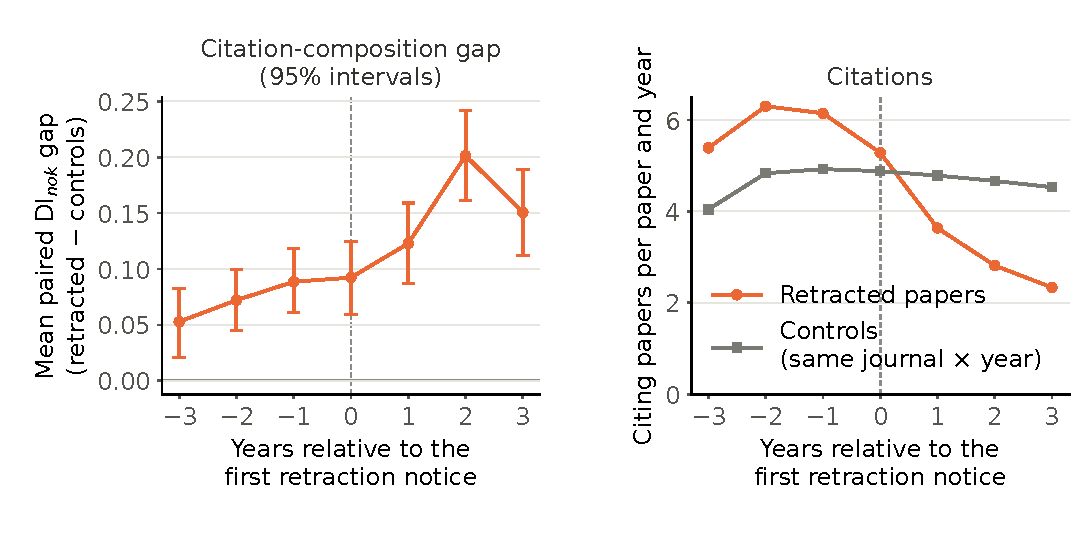
\includegraphics[width=\linewidth]{fig2_event}
\caption{The papers citing retracted papers around the first retraction notice (post hoc; 3,083 papers from
2000--2019 retracted between three years after publication and 2019, notice records excluded). Left: mean paired
annual DI$_{nok}$ gap, each retracted paper minus its same-journal--year control mean, with 95\% intervals from
2,000 bootstrap resamples of strata. Positive values mean papers that cite a retracted paper are less likely to also
cite its references than are papers citing its controls. Only defined pairs contribute; their numbers vary by year (\ref{sec:appendix}).
Right: citing papers per paper and year, including zero counts, in this balanced population, not the broader
5,100-paper window comparison.
Claude Opus 5.5 (Anthropic) assisted plotting code; GitHub Copilot CLI 1.0.116 (GitHub) assisted code and layout
revisions. The plotted values come directly from the reproducible analysis records.}
\label{fig:event}
\end{figure}

\section{Discussion}\label{sec:discussion}

\paragraph{A small mean difference, but a sign shift} For the late-retracted primary set, the post hoc 90\% interval
rules out absolute mean CD$_5$ differences above 0.00093, about 28\% of the review comparison's effect. Retracted papers
reach the top 5\% of their year about as often as controls, but positive scores are more common (odds ratio 1.23).
Thus, the two primary estimates do not give identical conclusions: the index registers a sign shift without a large
mean difference or unadjusted top-tier excess. An evaluation rewarding high CD$_5$ does not systematically favour
these late-retracted papers, but it does not exclude them either. A separate prospective study found that links to
papers retracted by a fixed cutoff predicted later retraction, albeit weakly as a standalone screen
\citep{arjomandi2026prospective}; \citet{lou2026beyond} reported the retrospective citation-network association.

\paragraph{What the $n_k$ term hides} The papers that cite retracted papers less often also cite their references.
The difference is small, three percentage points in the share of such citing papers or about 0.12 standard deviations
of DI$_{nok}$, but its point estimate is positive in every reason class, though near zero for honest error.
Its interval excludes zero for
misconduct and for other reasons, and the shift in its sign survives adjustment for reference and citation counts.
CD$_5$ registers it only through its sign, because the papers that cite only the references outnumber the citing papers
by more than two orders of magnitude for the median paper. The pattern is in line with the first expectation set out in
the introduction, that fabricated or falsified findings are cited without the literature they built on, but two other
readings fit the data and cannot be separated here: retracted papers may attract citations from outside their immediate
literature, or their reference lists may matter less to the papers that cite them. The data give no support to the
second expectation, that paper-mill products are consolidating. Whatever the reason, variants that remove $n_k$
\citep{wuyan2019solo,bornmann2020convergent} or that adjust for reference length would score retracted papers somewhat
higher than comparable papers. \citet{scancar2026distortion} found citation patterns among suspected paper-mill
articles in highly ranked molecular-cancer journals consistent with citation inflation. This motivates considering
the composition of citing papers, but does not establish why they omit a focal paper's references. The present
analysis does not exclude citing papers that are themselves retracted, so it cannot separate that possibility from
the other explanations.

\paragraph{Reference length and the top tier} At equal reference length, retracted papers reach the top 5\% of
CD$_5$ more often (odds ratio 1.42). The unadjusted comparison, which is what an evaluator sees, shows no
over-representation. The new matched mean-log reference difference, $+0.084$ (0.058--0.109), supports a reference-length
imbalance in the direction that suppresses high scores, consistent with the change after adjustment. The
adjusted estimate shrinks when citations in the window are also held fixed (1.19), but citations are part of the score
itself, so that model may over-adjust. These exploratory models show that the top-tier comparison is sensitive to
reference length; they do not establish a causal effect or validate a preferred adjustment.

\paragraph{Scores that include the retraction} Scores computed over windows that include the retraction differ for two
reasons. Notice records are counted among the citing papers, and more than a third of the papers retracted inside the
window have one. Beyond notices, the papers citing a retracted paper increasingly ignore its references while its
citations fall. This divergence starts before the notice, most clearly for misconduct, which fits critical attention
that precedes a formal retraction, and it steepens after the notice; the comparison is descriptive, not causal. For
users of the index the implication is simple: scores of retracted papers that include the notice year or later years
describe the retraction as much as the paper. They should be computed on a window that ends before the notice, with
notice records excluded, or be flagged.

\paragraph{Honest error} Papers retracted for honest error score slightly lower than their controls on CD$_5$, show no
clear difference on DI$_{nok}$, and their change after the notice shows no sign of an earlier trend. These classes are small (294
and 615 papers in the two windows), so the pattern should be read as a hypothesis: papers later found to contain errors
may build closely on their references, and their errors may come to attention only with the notice.

\paragraph{Relation to the debate on declining disruption} Requiring at least one reference removes almost all
CD$_5 = 1$ records (0.04\% remain), which are the records at the centre of the artefact debate
\citep{holst2024artefacts,holst2026partially,park2026reply}. This study makes no claim about long-run trends; the
yearly means of the reference sample are reported for orientation only. The size of $n_k$ found here, at least 90\% of
the denominator for almost all papers, is a reminder that CD$_5$ values near zero are the rule on a large citation
graph, so that differences between groups appear in thousandths.

\paragraph{Limitations} OpenCitations does not cover all references, and the choice of data source affects disruption
scores \citep{xu2025alternative,crossdi2025}; scores computed here are scores on open data. 83.3\% of Retraction Watch
papers were matched to the graph. Reason classes are a rule-based grouping of Retraction Watch reasons, and many
notices give limited information (the ``other'' class). Because the graph is complete only to about September 2023, the
main analysis ends with papers from 2017 and covers only 276 paper-mill papers; the post hoc three-year window raises
this to 708, but most paper-mill papers were published after 2019. Retractions are a selected and incomplete label of
problematic work: some unreliable papers are never retracted, and the controls may contain them. Several analyses
were added after the main results were known. Their plans were recorded before their runs, but the analyses remain
exploratory. The 0.00093 bound is an interval-based description, not a validated negligible-effect threshold.
Bootstrap resampling clusters by journal--year, not by author; serial retractors can contribute papers across
strata, so uncertainty may be understated if their outcomes are correlated. The diagnostic inputs contain no
author identifiers, preventing an author-cluster or largest-retractor exclusion check.
The primary set is also selected for late retraction: first notices occur in the sixth or a later calendar year after
publication. Its conclusions need not generalize to papers retracted during the scoring window, which are analysed
separately. Notice
records are identified only through PubMed. Because of the earlier trend, the change around the notice cannot be
attributed to the notice alone. Only two members of the index family are analysed.

\section{Conclusions}\label{sec:conclusions}

On the open biomedical citation graph, papers that were later retracted, including those retracted for misconduct and
paper-mill production, have a small mean CD$_5$ difference from comparable papers, and no unadjusted excess in the most
disruptive tier in the pre-specified five-year analysis. The post hoc three-year window leans toward a modest excess,
though this weakens under author-name exclusions. Positive scores are nevertheless more common, a sign shift that should not be read as complete
agreement between the groups. These conclusions concern papers retracted only after their scoring window.
The exploratory DI$_{nok}$ comparison shows what the index's largest term, $n_k$, compresses:
papers that cite a retracted paper are less likely to also cite its references. This difference persists after
removing notices, comments/letters and retracted citing papers, adjusting reference and citation counts, and
excluding the ten highest-retraction journals. A variant without $n_k$ therefore scores these late-retracted papers
somewhat higher than their controls. Scores that include retraction years behave differently again, through
notice records and a widening gap; scoring windows should end before the first notice, with notice records removed.
The analysis can be repeated with later snapshots of the open graph, which will add
the large cohorts of paper-mill papers published after 2019.

\appendix
\section{Exploratory diagnostics and accounting}\label{sec:appendix}
The identifiers P1--P12 refer to the archived plans in \texttt{POSTHOC.md}; the code's experiment index and
claim-to-run map link them to immutable results. These analyses were added after the primary results were known.

\subsection{Reference and citation counts (P1)}
The primary-set retracted papers have overall median reference counts of 40, against 35 for the full control pool,
and median window citations of 19 against 13. These pooled contrasts are not matched comparisons.
P1's within-stratum statistic first takes the group arithmetic mean count $m_{gs}$ for group $g$ in stratum $s$,
then computes $\log(1+m_{gs})$. Weighted by the number of primary retracted papers per stratum, the retracted-minus-control
differences are $-0.017$ for references and $+0.099$ for window citations. This is not the mean of the
paper-level $\log(1+\text{count})$ used in the conditional-logit models; P12 reports that matched quantity in the
main text. In the reference sample, CD$_5$ decreases with reference count (Spearman $\rho=-0.19$) and with window
citations ($\rho=-0.43$). The lower reference-count quartile is 29 for primary-set retracted papers and 22 for
the full control pool, not for a within-stratum comparison.

\subsection{Margins and interval interpretation (P3)}
P3 evaluates conventional margins with two one-sided tests
\citep{schuirmann1987tost,lakens2017equivalence}: $\pm0.1$ reference-sample standard deviations for mean differences
and 0.80--1.25 for odds ratios. The resulting mean margin, $\pm0.0044$, exceeds the observed review effect
($-0.0033$); the score SD is tail-sensitive, with a scored-set 5th--95th percentile span of about 0.028.
These margins are not validated negligible-effect thresholds for the index. This paper therefore interprets
the observed intervals and the 0.00093 bound, not equivalence to zero. The top-5\% odds ratio's 90\% interval is
0.85--1.16.

\subsection{Notice records (P8)}
In the CD$_5$ window, 36.7\% of papers retracted inside the window have a citing record identified by PubMed as a
retraction notice, erratum or expression of concern, against 4.7\% of the full control pool; so do 18.4\% of papers
retracted after the window. Removing notice records lowers the positive-score odds ratio from 1.71 (1.60--1.82;
5,861 compared papers) to 1.44 (1.34--1.54; 5,860 compared papers) for papers retracted inside the window,
and from 1.50 to 1.35 (1.28--1.43) for all retracted papers. The primary-set estimate changes little,
from 1.23 to 1.24 (1.14--1.34). These changes do not isolate the effect of the notice itself.

\subsection{Placebo timing and annual scores (P9 and P12)}
Among papers retracted at least four years after publication, a placebo notice three years before the real one
gives a difference in differences in DI$_{nok}$ of 0.036 (0.012--0.060; 2,565 compared papers), against
0.064 (0.037--0.093; 2,763 compared papers) for the real notice. By reason, the placebo change is close to zero
for honest error (0.005, $-0.065$ to 0.077; real notice 0.079, 0.012--0.149) but not for misconduct
(0.042, 0.010--0.074; real notice 0.078, 0.041--0.115).

Figure~\ref{fig:event} uses the balanced population with annual calendar coverage from three years before to three
years after the notice. P12 estimates the mean paired annual gap and its 95\% strata-bootstrap interval.
At event years $-3,-2,-1,0,1,2,3$, respectively, the numbers of defined pairs are
2,220, 2,504, 2,468, 2,440, 2,225, 1,982 and 1,854. Missing annual DI$_{nok}$ scores are not replaced by zero.
Mean control citations in this population range from 4.0 to 4.9 per year; it is distinct from the 5,100-paper
three-year-window comparison.

\subsection{Denominator size (P10)}
For the median scored paper, 2,862 papers in the window cite only its references, against 12 that cite the
paper itself. The $n_k$ term accounts for at least 90\% of the CD$_5$ denominator for 97.9\% of papers.
Thus a citation-composition difference can change the sign while producing only a small difference in CD$_5$.

\subsection{Controls behind the primary comparisons (P11)}
The 52,147 controls were drawn for all 10,450 retracted papers. The CD$_5$ primary comparison uses 2,239 strata
with 4,586 scored retracted papers and 31,674 controls, of which 12 have undefined scores, leaving 31,662.
The remaining controls belong to strata without a primary retracted paper in the comparison.
Pooled shares in the used strata are 18.1\% positive (5,725/31,662), 3.3\% above the top-5\% threshold
(1,047/31,662), and 0.56\% above the top-1\% threshold (176/31,662).
Weighting each stratum by its compared retracted papers instead gives 17.3\%, 3.1\% and 0.54\%, the shares
reported in the main comparisons. CD$_3$ uses 7,349 scored primary papers and 48,044 scored controls in 3,308 strata.


\section*{Data and code availability}\label{sec:availability}
% Public companion repository is built by ../../release/build_release.sh.
Citation data: \citet{arjomandi2024dataset}; identifiers, years and journals: \citet{ocmeta2024dump}; retractions:
the Retraction Watch database distributed by Crossref (repository commit of 30 October 2026), linked to the graph as
published in \citet{arjomandi2026retracteddata}; PubMed 2026 baseline courtesy of the U.S. National Library of
Medicine. Scripts, the specification files with their recorded hashes, run records with checksums, the aggregate result
tables and a map from every number in this article to the run that produced it:
\ifanon [repository link removed for anonymized review]\else
\url{https://github.com/HosseinMA96/retracted-disruption-open-data}\fi. Per-paper scores of non-retracted papers are
not released. This is a reporting choice, not a restriction imposed by the source data: scores could be mistaken for
paper-level integrity labels, so only aggregate comparisons are published for non-retracted papers. All source data
and scripts needed to recompute those scores are identified above and in the repository.

\paragraph{Pre-specification record} The unchanged specification is \texttt{SPEC.md}, committed in the private
project repository on 10 November 2026 at 04:02:19 UTC (Git commit
\texttt{293755b1cb7087d6f226d6f96f4b97cb0148e4c5}). Its full SHA-256 is recorded in the public
\texttt{spec\_provenance.json} and the score run's \texttt{run.json}, which reports a start time of 06:12:02 UTC the same day
(\texttt{e03\_cd5\_20261110\_01}); the evaluation run records the same hash. These files and provenance are available
with the code, but the original repository and its commit history remain private: the cited commit cannot be
inspected through the public release. The public provenance file reports this limitation explicitly.
Git dates and run records describe the claimed ordering, not an independently verifiable registry timestamp.
VM analysis and laptop figure/Git records use different system clocks; cross-host timestamp strings are not
directly comparable. Clock sources and discrepancies are documented in \texttt{spec\_provenance.json}.
The design is described as pre-specified, not publicly pre-registered.
The citing-record/journal sensitivity was recorded after the original results and published before execution in
\href{https://github.com/HosseinMA96/retracted-disruption-open-data/commit/9c4ba4ca9bca39542f86a014bda2db463c1534ac}{the public P15 plan commit}.
The identifier-aware type audit, major-MeSH matching and fixed-window interval rules were likewise recorded in
\href{https://github.com/HosseinMA96/retracted-disruption-open-data/commit/018d835f7db497a788320977d54d4b62f3755918}{the public P16 plan commit}.


\section*{Declaration of generative AI and AI-assisted technologies in the manuscript preparation process}
% Elsevier recommended wording (policy page read 2026-11-23); research-process use is described in Methods
% ("Software and AI assistance"). Original tool list confirmed by the author on 2026-11-26.
During the preparation of this work, the author used Claude Opus 5.5 (Anthropic) in order to search and summarize the
literature, draft and edit the text, and write analysis and figure scripts under the author's direction.
The author designed the study and specified every analysis, including the exploratory checks; AI tools assisted
implementation and manuscript preparation.
GitHub Copilot (powered by GPT-6.1 Sol, OpenAI) was used to write and test additional analysis code, update figures,
and check and edit the manuscript before submission. After using these tools, the author reviewed and edited
the content as needed, checked numerical claims against analysis outputs, reviewed the analysis code and
methodological choices, and checked cited sources against the manuscript claims.
The author takes full responsibility for the content of the
published article.


\section*{Declaration of competing interest}
The author declares no competing interests.

\section*{Funding}
This research did not receive any specific grant from funding agencies in the public, commercial, or not-for-profit
sectors.

\ifanon\else
\section*{CRediT authorship contribution statement}
\textbf{Hossein Mohasel Arjomandi:} Conceptualization, Methodology, Software, Formal analysis, Data curation,
Visualization, Writing -- original draft, Writing -- review \& editing.

\section*{Disclaimer}
The views expressed in this article are the author's own and do not necessarily reflect those of Microsoft.
\fi

\bibliographystyle{elsarticle-harv}
\bibliography{../../refs}
\end{document}
